\chapter{Problem Formulation}
\label{capitolo3}
\thispagestyle{empty}

\section{The Utility of Doors Detection for Mobile Robots}

As mentioned in the previous chapter, doors are useful semantic features for an active agent. Collecting information about doors, a robot improves significantly its knowledge about the environment in which it operates. Exploration and navigation, two of the main task for a mobile robot, can be strongly influenced by doors data, such as their location and status (e.g. closed or opened). Exploration, the task in which an autonomous agent incrementally discovers feature of interest in an initially unknown environment, can be considered for map building.  The map acquisition enables autonomous agents to navigate inside a previously unknown environment. This procedure allows the robot to build a metric map of the indoor environment it is exploring. Typically, a metric map is a occupancy grid map, a two dimensional matrix in which each cell, that represents a sub-portion of the environment, contains the probability that it is occupied by an obstacle. It define a spatial representation of environments, describing the probability to meet an obstacle in a certain location. Occupancy grids were first proposed in \cite{cuupancygridfirst} and they being widely used for mobile robot localization, exploration, and navigation \cite{gridmapnavigation, ariel, girdmapexploration}. A way to store and visualize occupancy grid maps is to encode it in an 8-bit gray-scaled image, normalizing the probability values of the cells to the range between 0
and 255. A further simplification consists are binary occupancy grids (Fig. \ref{fig:binary_grid_map}), where each cell has a boolean value representing the occupancy status. An occupied location is represented as \textit{True} (1) and a free location is represented as \textit{False} (0). Collecting data about doors can improve the mapping strategy followed by mobile robots. By detecting closed doors, an agent guess that some floor areas are temporarily unreachable, and can consequentially act to collect the entire environment map. For example, it can open the door through a robotic arm \cite{doorcabinet} or asking help to a human operator. Another solution concerns identifying the presence of unreachable locations by detecting closed door and making a map refinement in future stages (when closed doors have been opened).

Room segmentation divides grid maps into semantically meaningful regions making the pure spatial environment model, provided by grid maps, more informative. Fig. \ref{fig:room_segmentation_map} shows an occupancy grid map divided in rooms. \citeauthor{segmentationsurvey}, \cite{segmentationsurvey}, survey the literature on room segmentation and provide a comparison of the most relevant methods. They argue that room segmentation yields significant savings in computational efforts for obtaining navigation trajectories \cite{segmenationfornavigation}. Likewise, human-robot communication greatly benefits from an high level room's division \cite{segmentationhumanrobot}. Furthermore, cleaning agents can exploit room maps to improve its navigation strategy, creating an efficient cleaning path throughout the floor plan \cite{segmentationcleaning}. While spatial mapping have been extensively investigating and several automatized tools have been proposed to solve them, the research community is still investigating robust methods for obtaining accurate room-level segmentation of an indoor environment. The sensors' technology is imperfect, so noise and missing data introduce several errors in robot perception. Furthermore, indoor environments are highly cluttered with furniture and other objects. Separating clutter from permanent structures such as walls and doors is difficult as furniture can occlude important structural features. Robust doors detection can improve the grid maps segmentation providing useful information of connections between different rooms.

\begin{figure}[h!]
	\centering
	\begin{subfigure}[b]{0.5\linewidth}
		\centering
		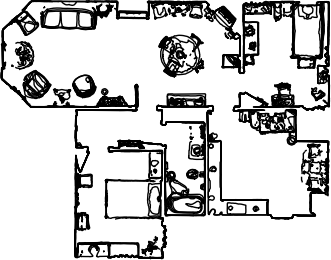
\includegraphics[width=\textwidth]{images/occupancygrid.png}
		\caption{Binary occupancy grid map.}
		\label{fig:binary_grid_map}
	\end{subfigure}
	\hfill
	\begin{subfigure}[b]{0.45\linewidth}
		\centering
		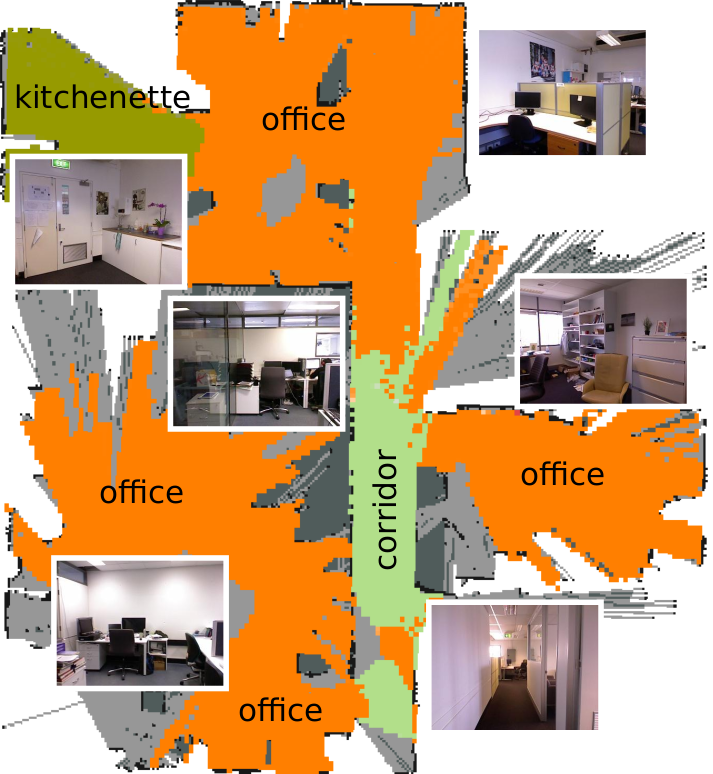
\includegraphics[width=\textwidth]{images/semanticmap.png}
		\caption{Semantic map \cite{placecategorization}.}
		\label{fig:semantic_map}
	\end{subfigure}
	\newline
	\newline
	\begin{subfigure}[b]{0.99\linewidth}
		\centering
		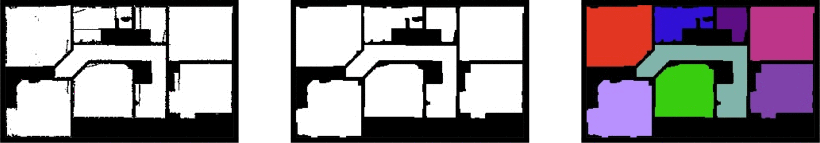
\includegraphics[width=\textwidth]{images/roomsegmentation.png}
		\caption{Room segmentation map \cite{segmentation3d}.}
		\label{fig:room_segmentation_map}
	\end{subfigure}
	\caption{Three different types of maps.}
	
\end{figure}

The room level map obtained through room segmentation can be further improved exploiting scene recognition or place categorization. This task consists on identifying indoor scenes, such as an office, a kitchen, or a bedroom. Through place categorization an autonomous agent builds a semantic map (an example is shown by Fig. \ref{fig:semantic_map}), in which any environment location is tagged with a semantic label. In literature there are a lot of studies concerning place categorization by autonomous agents \cite{scenerecognitionaudio, scenerecognitiononjectdetection, placecategorization, placecategorizationlargescale}. The goal is to build a semantic map that indicates the type of each place in an indoor environment. These approaches collect useful information from the environment (like audio signal or RGB images), then classify these data to divide the environment in rooms, and finally assign a semantic label to each place. One of the main problem is to correctly segment the environment in rooms. This is because data acquired in different rooms can be similar (in this case adjacent rooms can be considered as the same semantic place) or the same room can present different features that may produce a split in separate semantic places. Identifying the connection between rooms, represented by doors in an indoor environment, and estimating their location allows to robustly identify different semantic rooms in an indoor environment. Furthermore, doors detection can helps this methods to find the precise location in which a semantic place ends and another room begins, building more refined place segmentation and categorization.  

Another task that can get benefit from doors detection is Semantic SLAM (Simultaneous Localization and Mapping). Semantic SLAM aims to build a semantic map online during exploration, without a complete and previously-acquired knowledge of the environment. Recent Semantic SLAM methods combine classical geometry-based estimation with deep learning-base object detection. The work presented in \cite{semanticslamsurvey} surveys and evaluates the most relevant approaches to perform Semantic SLAM. The authors argue that semantic segmentation is the largest source of error in the analyzed methods. Doors are useful semantic features of indoor environments and their detection can be added in Semantic SLAM approaches. Furthermore, the doors detection can be used to improve the segmentation accuracy performed in previous stages, because the robot can group the data acquired in different rooms of the same environment. 

\section{Goals}

This thesis presents a module to perform doors detection by autonomous mobile agents. Researchers propose feature based methods \cite{sonarandivisualdoordetection, humanoid, edgeandcornerdoorsdetector} and deep techniques \cite{detectdoorsfeature, doorsandnavigation, doorcabinet} for detecting door in indoor environments.  The module proposed in this work uses RGB images as input data, approaching the problem as an object detection task. Computer Vision is highly dependent on the power of deep learning and the novel transformers-based architectures for object detection obtain competitive results compared with previous techniques. Since the peculiarities of transformers have not yet been tested in a doors detection task, the proposed detector is based on DETR \cite{detr}: a deep end-to-end module that take advantages of Transformers to capture the relationships between visual features vectors extracted by a CNN backbone. 

The development and training of a deep module used in a robotic vision context has to be more general as possible. This is because, in the subsequent deployment phase, an agent operates in an unknown environment. The model's performance can greatly degrade in unfamiliar scenes, since their features and structural characteristics have not been considered during the training phase. Despite this, an autonomous agent operates in a few environment during its life cycle. Intelligent agents, like service robots or smart vacuum cleaners, are deployed in a specific environment and often operates inside it during all their life cycle. Frequently moving a robot from an scene to another is not a common scenario. Intelligent agents implement complex strategies for orienting and navigating in real environments. As robots try to understand a scene as well as possible, also artificial environments offer some feature and structural elements that helps agents' perception. Researches defined the \textit{wayfinding} principle, which encompasses all of the ways in which people (and animals) orient themselves in physical space and navigate from a place to another. Following this knowledge of how human perceive, architects design and build artificial environment that helps human to orient and navigate inside it. In \citeyear{imageofcity}, \citeauthor{imageofcity} introduced this concept in his book \citetitle{imageofcity}, where \textit{wayfinding} is defined as ``a consistent use and organization of definite sensory cues from the external environment''.  The author argue that, in the process of \textit{wayfinding}, the strategic link is the generalized mental image of the exterior physical world that is held by an individual. The coherence of the image may arise in several ways. For example, objects can be ordered or remarkable in a scene, so the user recognizes them through its previous experience and the familiarity acquired with the environment. Alternatively, an object seen for the first time may be identified because it
conforms to a stereotype already constructed by the observer in other scenes. In \citeyear{wayfinding}, the \textit{wayfinding} concepts were further expanded from \citeauthor{wayfinding} in their book entitled \citetitle{wayfinding} \cite{wayfinding}. This works describes and illustrates how people use both sings and other wayfinding cues to find their way in complex scenes, all set into practical contexts. 
Indoor environments presents a coherent design and a standardized visual aspect in order to help \textit{wayfinding} strategies used by intelligent agents. Following this intuition, in the same environment there are a few types of doors, repeated in different locations. The intuition of this thesis is to imply the \textit{wayfinding} characteristics of indoor environments (originally realized for humans) in a robotic vision task to increase the detection performance. Considering the deployment condition of mobile robots (agents operates in the same territory for a long time) and the coherent design of indoor environments, this work propose an approach for increasing the doors detector accuracy in unfamiliar environments. The main idea is to specialize the previously trained general doors detector on the specific environment in which the robot operates. This method, called \textit{one-shot incremental learning}, consists on collecting a sub-set of examples from the unfamiliar scene in which the robot will be deployed. Then, the detector is re-trained using these new environment-specific data. In this way, the doors detection module learns how to robustly recognize the new types of doors that characterize the deployment environment. Furthermore, this thesis investigates the amount of data required to achieve an acceptable increase in performance.

The power of deep learning is limited in vision robotics applications by some problems and challenges that researchers are still investigating. The datasets used in computer vision tasks are not suitable for robotic vision applications. They do not contain sufficient data to well generalize the domain they represent. Objects of the same category can look very different depending on the context in which they are use and the scene's design, so the examples must to be collected from several environment types. Due to a mobile agent can autonomously explore an area, the object images to train a deep robotic detector must be captured from different viewpoints. Furthermore, the locations from where data are acquired should be consistent with a possible exploration strategy followed by a mobile robot. In addition to datasets, even metrics used in computer vision are insufficient to evaluate an end-to-end robotic vision module. They compute an overall statics over a single dataset which often includes only positive samples (images with objects to detect). To overcome the limitations just mentioned, this thesis describes a method for acquiring a visual dataset specific for door detection in a robotics context. The examples are collected in virtualized heterogeneous environments scanned from real world. The viewpoints are chosen simulating an exploration strategy plausible for an active agent. Furthermore, this thesis proposes a novel evaluation method that considers also the negative samples (images without doors to detect).

\section{Problem Description}

Before proceeding with the detailed discussion of our work, we firstly report some definitions and concepts about the problem addressed by this thesis. In the following paragraphs, we define the ideal deployment scenario in which an autonomous agent can benefit from the proposed method. Furthermore, we define the concept of door considered by this thesis, specifying the status that they can assume and the data used to their recognition.

\subsection{The Ideal Deployment Scenario}

This thesis proposes a method to improve the accuracy of a door detector module used by autonomous agents. The most intuitive way to reach this goal is to focus only on the module that performs doors detection. This idea consists on building a doors detector more robust as possible, choosing the most suitable technique proposed by the state-of-the-art and optimizing it for this specific object category. Improving the module which performs detection can be a good choice, but other important aspects can be considered to this end. The method proposed by this work aims to increase the doors detector's accuracy in a specific deployment scenario of mobile robots. Indoor agents, such as service or healthcare robots, intelligent housekeepers, and smart vacuum cleaners, are developed to operate in any environment type. This is because the final context in which a robot works is unknown and it can vary a lot. For example, an healthcare agent can be employed in an hospital or in a retirement house. Service robots can be used in a luxury home or in a restaurant, while a smart vacuum cleaner can operates in a flat or in a refectory. Each environment type has its own structural characteristics that vary a lot from each others. Furthermore, built environments of the same type can have a completely different design or visual aspect, depending on the construction budget or on the occupants' culture. For example, an house near the sea is extremely different from a mountain house. During the development phase, it is difficult make assumption on the type and on the most relevant visual and structural features of the environment in which a robot is deployed. This is because an autonomous agent must be developed in a general way, in order to be suitable for every environment in which it finally operates. Despite this, an indoor mobile robot is typically deployed in a single environment and operates inside it throughout its life cycle or, otherwise, for a long time. This is the ideal deployment scenario considered by this thesis. We consider the case in which a robot, to exploit its assigned task, navigates the same environment and finds doors to improve its reasoning abilities. The main idea is to specialize a general module that performs doors detection to a single specific environment, in order to improve its performance. In the context of this thesis, we take into account only indoor environments. In particular, they are an heterogeneous set of multi-floor houses, in which each environment has a particular interior design and a different visual aspect, top better generalize the problem. Furthermore, we assume the environments are static, i.e. their structural features don't change during exploration.

\subsection{Door's Definition and Data Used} 

The second set of definitions we make is about the concept of doors and the data used by the detector to find them. The authors of the work presented in \cite{topologyurban} define the concepts of \textit{portal}, which is located whenever a pair of different spaces are adjacent and no physical barriers prevent direct traversal between them.  A portal can be \text{vertical} or \textit{horizontal}. The first type of portals connects adjacent floors in the same indoor environment (such as stairs, elevators or ramps), while the latter unifies a tuple of locations on the same floor. The authors identify two types of horizontal portals: \textit{explicit} and \textit{implicit}. Explicit portals are connections between two adjacent spaces separated by a barrier (e.g. a doorway through a wall), while implicit portals represent connections between spaces with no physical barrier. In the context of this thesis, we consider doors as implicit and explicit horizontal portals. In particular, explicit doors are composed by a jamb and a leaf. Otherwise, implicit doors do not have these components, typically they are only holes in walls that connects different spaces in the same environment. We consider both \textit{internal} and \textit{external} doors. The first are connections between two different spaces inside the same environment while the latter lead out of the building. The method proposed by this thesis not only detect doors, but only their status. A door can be \textit{open} or \textit{closed}. A door is closed door when the door leaf is completely resting on the jamb, while a door is considered open it presents even a little hole. We do not consider any other intermediate state (e.g. semi-opened) and do not define how much a door is opened. It is important to specify that only explicit doors can assume both status, while implicit ones are always open. The approach we describe in this thesis detects door from RGB images. An image is a $n \times n$ matrix in which each cell is called pixel. Each pixel is composed by three 8-bit values that represent the color using the RGB encoding. It is an additive color model in which the red, green, and blue primary colors of light are added together in various ways to reproduce a broad array of pigments. Doors are highlighted in images by drawing a rectangular bounding box around it.

\begin{figure}[h!]
	\centering
	\begin{subfigure}[b]{\linewidth}
		\centering
		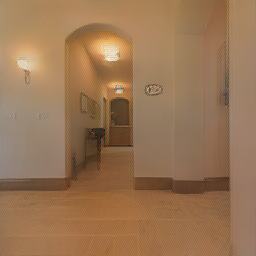
\includegraphics[width=0.24\textwidth]{images/implicitdoor1.png}
		\hfill
		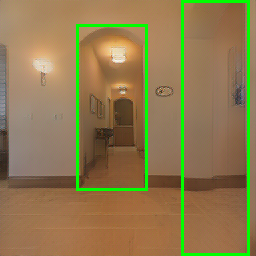
\includegraphics[width=0.24\textwidth]{images/implicitdoor1boxed.png}
		\hfill
		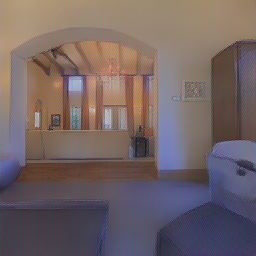
\includegraphics[width=0.24\textwidth]{images/implicitdoor2.png}
		\hfill
		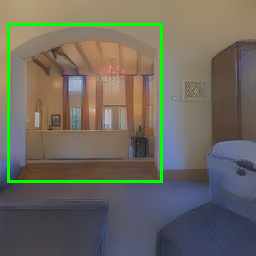
\includegraphics[width=0.24\textwidth]{images/implicitdoor2boxed.png}
		\caption{Implicit internal open doors and the relative bounsing boxes.}
	\end{subfigure}

	\begin{subfigure}[b]{\linewidth}
		\centering
		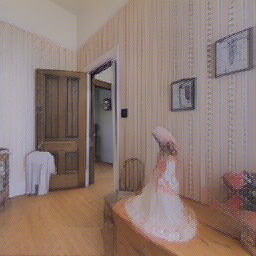
\includegraphics[width=0.24\textwidth]{images/explicitinternalopen1.png}
		\hfill
		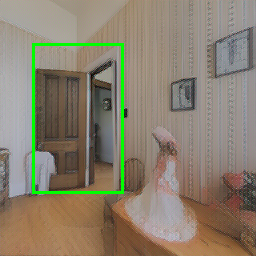
\includegraphics[width=0.24\textwidth]{images/explicitinternalopen1boxed.png}
		\hfill
		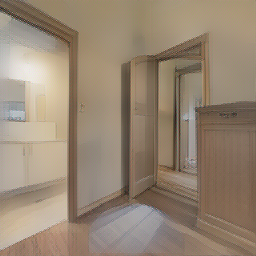
\includegraphics[width=0.24\textwidth]{images/explicitinternalopen2.png}
		\hfill
		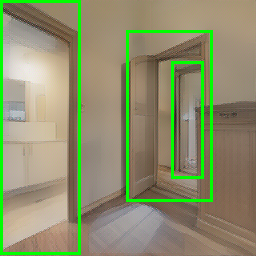
\includegraphics[width=0.24\textwidth]{images/explicitinternalopen2boxed.png}
		\caption{Explicit internal open doors and the relative bounsing boxes.}
	\end{subfigure}

	\begin{subfigure}[b]{\linewidth}
		\centering
		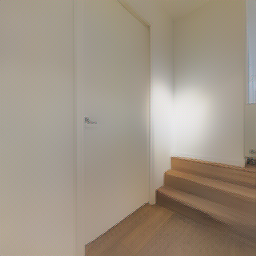
\includegraphics[width=0.24\textwidth]{images/explicitinternalclosed1.png}
		\hfill
		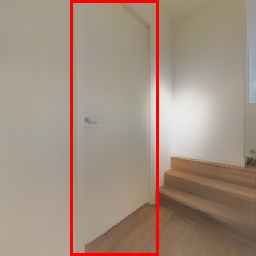
\includegraphics[width=0.24\textwidth]{images/explicitinternalclosed1boxed.png}
		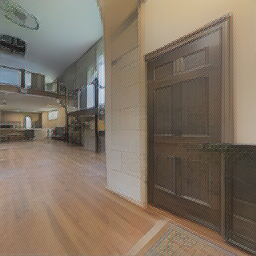
\includegraphics[width=0.24\textwidth]{images/explicitinternalclosed2.png}
		\hfill
		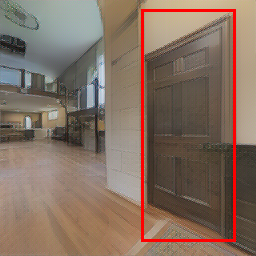
\includegraphics[width=0.24\textwidth]{images/explicitinternalclosed2boxed.png}
		\caption{Explicit internal closed doors and the relative bounsing boxes.}	
	\end{subfigure}
	
	\begin{subfigure}[b]{\linewidth}
		\centering
		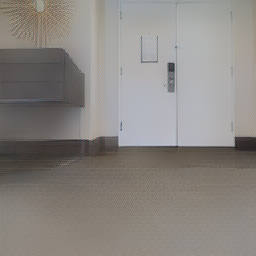
\includegraphics[width=0.24\textwidth]{images/explicitexternalclosed1.png}
		\hfill
		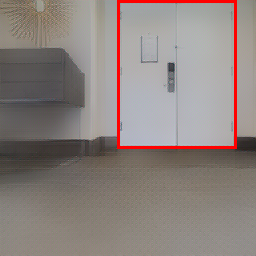
\includegraphics[width=0.24\textwidth]{images/explicitexternalclosed1boxed.png}
		\hfill
		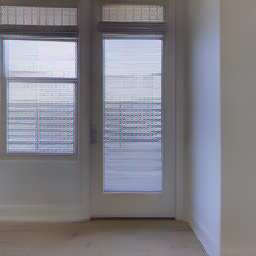
\includegraphics[width=0.24\textwidth]{images/explicitexternalclosed2.png}
		\hfill
		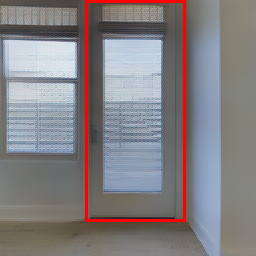
\includegraphics[width=0.24\textwidth]{images/explicitexternalclosed2boxed.png}
		\caption{Explicit external closed doors and the relative bounsing boxes.}
	\end{subfigure}
	\caption{Different types of doors. Green bounding boxes represent open doorways while red rectangles denote closed doors.}
\end{figure}

